\documentclass[a4paper]{article}
\usepackage{graphics}
\usepackage{tikz}
\usepackage{xifthen}
\usepackage{xstring}

% Modified version of https://www.latex4technics.com/?note=3twf
\newcommand{\randomwords}{%
  radar; frequency; waves; ocean; spectrum; transformation; beam; reflection; energy; roughness;
  amplitude; shift; Doppler; antena; detection; crest; equation; integral; domain; component;
  crossection; interaction; reconstruct; crystal; lattice; atomic; signal; probability; density; application;
  peak; intensity; coherent; structure; transmission; image; noise; filter; distance;
  observations; oscillations; error; measure; absorb; target; distribution; mrean; deviation; smooth
}
\usepackage{datetime}
\pgfmathsetseed{SEED}  % This is a template file 

\pgfmathsetmacro{\cellsize}{2}
\pgfmathtruncatemacro{\gridsize}{5}

\pgfmathtruncatemacro{\fieldcount}{\gridsize*\gridsize-1}
\pgfmathtruncatemacro{\bingo}{\fieldcount/2}
\StrCount{\randomwords}{;}[\numwords]
\newcounter{myletter}
\pgfmathtruncatemacro{\minusgrid}{\gridsize-1}

\pagenumbering{gobble}



\begin{document}



\begin{center}\Large{
    Susanne's Trial Lecture Bingo
}\end{center}

\begin{figure}[h!]
  \begin{center}
\begin{tikzpicture}[scale=1, every node/.style={scale=1}]
  \foreach \f in {0,...,\fieldcount}
           { \pgfmathtruncatemacro{\x}{mod(\f,\gridsize)}
             \pgfmathtruncatemacro{\y}{div(\f,\gridsize)}
             \pgfmathtruncatemacro{\mycolor}{mod(\f,2)*100}
             \draw[fill=blue!\mycolor!yellow!20] ({\x*\cellsize},{\y*\cellsize}) rectangle
             ({(\x+1)*\cellsize},{(\y+1)*\cellsize});
             \ifthenelse{\f=\bingo}
                        {\node[] at
                          ({(\x+0.5)*\cellsize},{(\y+0.5)*\cellsize}) {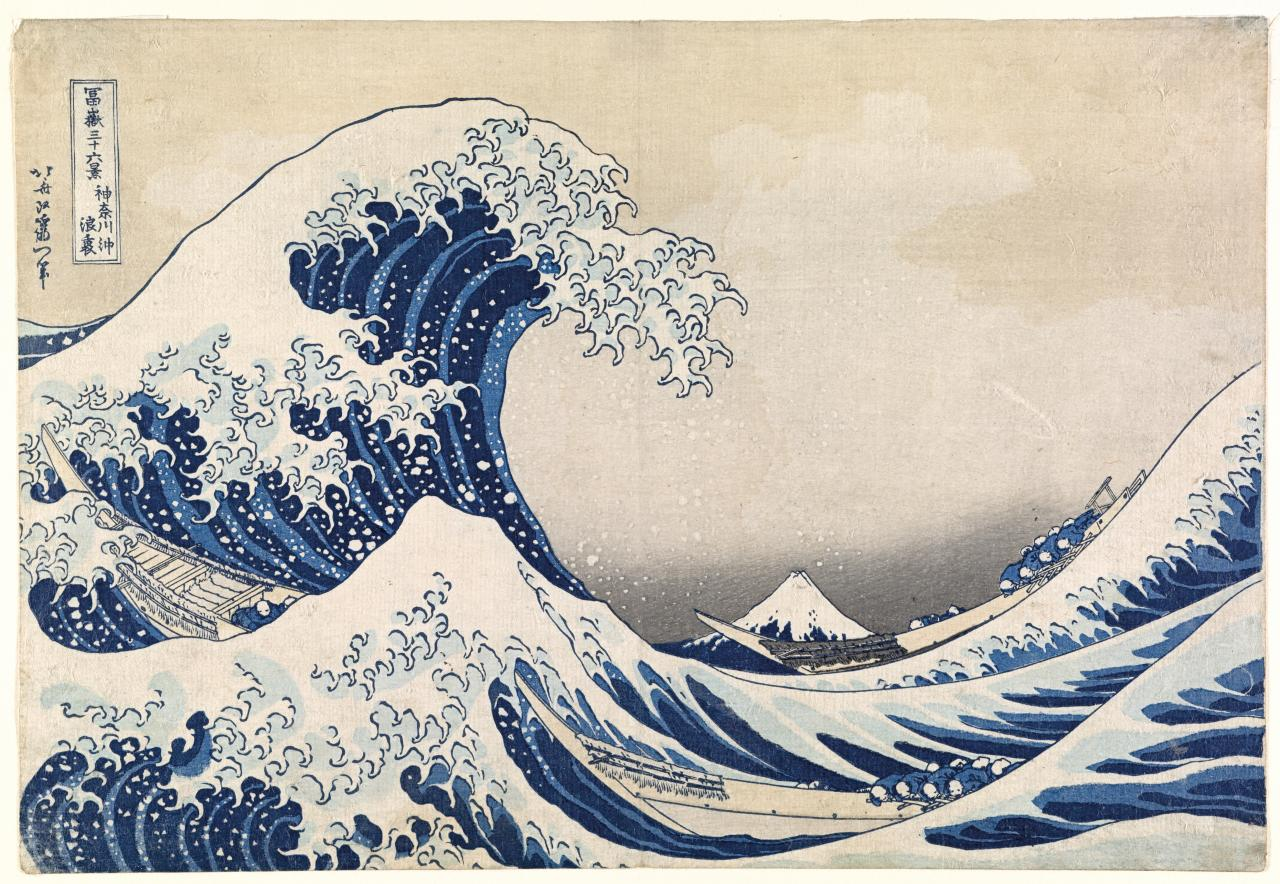
\includegraphics[width=0.16\textwidth, height=0.16\textwidth]{freak_wave.jpg}};
                        }
                        { \pgfmathtruncatemacro{\maxvalue}{\numwords-1-\f)}
                          \pgfmathtruncatemacro{\myrandom}{random(\maxvalue)}
                          \pgfmathtruncatemacro{\mynextrandom}{\myrandom+1}
                          \StrBetween[\myrandom, \mynextrandom]{\randomwords}{;}{;}[\randomword]
                          \StrDel{\randomwords}{\randomword;}[\randomwords]
                          \xdef\randomwords{\randomwords}
                          \node[rotate=45] at ({(\x+0.5)*\cellsize},{(\y+0.5)*\cellsize}) {\randomword};
                        }
                        \ifthenelse{\x=0}
                                   {\draw[fill=red!10!white]
                                     ({\x*\cellsize},{\y*\cellsize}) rectangle
                                     ({(\x-0.5)*\cellsize},{(\y+1)*\cellsize});
                                     \node at
                                     ({(\x-0.25)*\cellsize},{(\y+0.5)*\cellsize})
                                           {\pgfmathparse{int(\gridsize-\y)}\pgfmathresult};
                                   }{}
                                   \ifthenelse{\y=\minusgrid}
                                              {   \draw[fill=red!10!white]
                                                ({\x*\cellsize},{(\y+1)*\cellsize}) rectangle
                                                ({(\x+1)*\cellsize},{(\y+1.5)*\cellsize});
                                                \pgfmathparse{int(\x+1)}
                                                \setcounter{myletter}{\pgfmathresult}
                                                \node at ({(\x+0.5)*\cellsize},{(\y+1.25)*\cellsize})
                                                      {\Alph{myletter}};
                                              }{}
           }
\end{tikzpicture}
  \end{center}
\end{figure}

\hrule
\vspace{2pt}
   \footnotesize{
     Rules: The game starts \emph{after} title slide and table of content
     slide. Freak wave is the ``joker card'' of the game. Do \emph{not} call
     out Bingo! Instead record the slide number where you got it; the first
     player with Bingo gets a prize.
    }

\end{document}
